\section{Slope limiting}
It is well known \cite{dolejsi2015} that the Discontinuous Galerkin method exhibits nonphysical spurious oscillations in the vicinity of sharp discontinuities. Noteworthy is the fact, that with continuous Finite Element spaces, the situation is even worse, as the oscillations tend to propagate through the computational domain. With the DG method, the problem is localized to a single layer of elements bordering any sharp front. This behavior is not acceptable, and measures must be taken to eliminate such oscillations - methods aiming at solving this are usually labeled as flux limiters, slope limiters, or shock capturing schemes.
\paragraph{}
These methods can be categorized according to multiple aspects. Out of these, two are important from the perspective of this work. First categorization is whether the approach changes the equations by introducing additional term that 'smoothes' the solution near the sharp front (this may be understood as a form of \textit{artificial viscosity / resistivity}) - such approach is proposed e.g. in \cite{DENNER201759}.
\paragraph{}
In this work, such an approach is not preferred, as we aim at implementing a generally usable solver, where extensive analysis of the impact of a change in the governing equations for the particular problem is not possible.
\paragraph{}
Second categorization worth mentioning is whether the particular approach is suitable for multi-scale phenomena, where the solution can exhibit large jumps in all possible configurations with respect to the (non-uniformly refined) mesh. From a pragmatic perspective, a rather simple slope and robust limiting technique that does not change the governing equations is the Barth-Jespersen limiter \cite{barthJespersen}.
The Barth-Jespersen limiter considers the piecewise-linear solution in the form
\be
\label{slopeLimSln}
u_h\lo x\ro = u_c + \alpha_e\lo\nabla u\ro_c \cdot \lo x - x_c\ro,\ 0 \leq \alpha_e\leq 1,
\ee
obtained using the linear Taylor basis functions (description of this shapeset is given in \cite{KuzminVertex}), where $u_c$ is the cell average on the element $K$, and $\lo\nabla u\ro_c$ is the gradient of the solution on the element $K$.
\paragraph{}
The sought parameter $\alpha_K$ is the parameter (correction factor) that determines the maximum admissible slope and is defined as:
\be
\alpha_K = \min_i\left\{\begin{array}{c}
\min\left\{1, \frac{u_K^{max} - u_c}{u_i - u_c}\right\},\ if\ \ u_i - u_c > 0,\\
1,\ \ \ \ \ \  \  \  \   if\ u_i - u_c = 0,\\
\min\left\{1, \frac{u_K^{min} - u_c}{u_i - u_c}\right\},\ if\ \ u_i - u_c < 0,\end{array}\right.
\ee
where $u_i = u_c + \lo\nabla u\ro_c \cdot\lo x_i - x_c\ro$ is the unconstrained solution value at the vertex $x_i$, and $u_K^{min}, u_K^{max}$ are the minimum and maximum cell averages of all elements sharing a common face with the element $K$.
\paragraph{}

However, using this limiting technique, there are two suboptimal behavior features - the bounds for the limited solution are set on one hand too tight - solution values from elements meeting at a vertex but having no common face are not taken into account (they might extend the interval for the admissible correction factor $\alpha_e$, and on the other hand too loose - solution values on elements that share a common face may extend the admissible interval for $\alpha_e$ based on the value at a vertex that does not belong to that particular common face.
\paragraph{}
Both these two problems are solved in the slope limiting technique chosen for this work
\subsection{Vertex-based limiter}
\label{sec:vertex}
Introduced by D. Kuzmin in \cite{KuzminVertex}, the Vertex-based limiter aims at being an improvement over the Barth-Jespersen limiter. It also considers the solution in the form \cref{slopeLimSln}, but the definition of the correction factor $\alpha_K$ differs:

\be
\label{vertexBasedAlpha}
\alpha_K = \min_i\left\{\begin{array}{c}
\min\left\{1, \frac{u_i^{max} - u_c}{u_i - u_c}\right\},\ if\ \ u_i - u_c > 0,\\
1,\ \ \ \ \  \  \  \  if\ u_i - u_c = 0,\\
\min\left\{1, \frac{u_i^{min} - u_c}{u_i - u_c}\right\},\ if\ \ u_i - u_c < 0,\end{array}\right.
\ee
where in this case $u_i^{min}, u_i^{min}$ are defined in such a way that for each of the vertices they are initialized with a small and a large constant, respectively, and then in the loop over all elements that contain the $i-$th vertex, the values are updated as:
\be
u_i^{max} = \max\left\{u_c, u_i^{max}\right\},\ \ u_i^{min} = \min\left\{u_c, u_i^{min}\right\}.
\ee
This slope limiting technique proves to have all the required attributes from the perspective of this work. The algorithm implementing this technique looks is presented in \cref{algorithm:limiter}

\begin{algorithm}[H]
	\# Loop over elements\\
	\ForEach{$K\in T_h$}{
		\# Loop over solution components\\
		\ForEach{$k = 1, ..., 8$}{
			\# In the rest of the algorithm, $u$ will stand for $u^k$.\\
			\KwData{Center value of the solution $u_c^K = u\lo x^K_c \ro$ at point $x^K_c$ which is the center of $K$}
			\KwData{Set of linear basis functions coefficients obtained as:}
			\# Loop over basis functions for the component $k$\\
			\ForEach{$v_1^k := v\in \left\{v\in v_h \lo {K} \ro, \text{component of } v = k,\ v \text{ piecewise linear} \right\}$}{
				\KwData{$l\lo v \ro$ - index of $v$ in the global system, i.e. row in \cref{Linear3} - \cref{Linear5}}
				\KwData{$u_{l\lo v \ro}$ - solution coefficient for $\lo v \ro$}
			}
			Set $\alpha_K = 1$\\
			\# Loop over vertices\\
			\ForEach{$v_i, i = 1, ..., 8, v_i$ is a vertex of $K$}{
				\KwData{Vertex value $u_i = u\lo v_i \ro$}
				\KwData{Set of vertex neighbors $\left\{K^{'}\right\}_i$, where $v_i \in K^{'}$ and $K^{'} \neq K$}
				\# Loop over elements sharing the vertex $v_i$\\
				\ForEach{$K^{'}\in \left\{K^{'}\right\}_i$}{
					\KwData{Center value of the solution $u_c^{K^{'}} = u\lo x^{K^{'}}_c\ro$ at point $x^{K^{'}}_c$ which is the center of $K^{'}$}
				}
				Calculate $u^{max}_i = \max\left\{u_i, \max\left\{u_c^{K^{'}}\right\}\right\}$\\
				Calculate $u_i^{min} = \min\left\{u_i, \min\left\{u_c^{K^{'}}\right\}\right\}$\\
				Evaluate \cref{vertexBasedAlpha}, updating $\alpha_K$
			}
			\ \\
			\# Loop over basis functions for the component $k$\\
			\ForEach{$v \in v_1^k$}{
					$u_{l\lo v \ro} = \alpha_K u_{l\lo v \ro}$
			}
		}
	}
\caption{Limiting the solution using the vertex-based limiter.}
\label{algorithm:limiter}
\end{algorithm}

\subsubsection{Comparison of limited and unlimited solution}
For illustration, the same problem as in \cref{subsec:numfluxcomp} is considered, which is suitable for illustrating the undershoots and overshoots, as the problem contains a sharp front where this behavior is clearly visible.
In the next Figures, first several snapshots of an unlimited solution, and then several snapshot of a limited solution are presented. Note that the unlimited solution can't progress beyond a certain point, as the undershoots and overshoots get so large that the density values get to be negative, therefore e.g. calculating its square root needed for the speed of sound evaluation is impossible. Even before that, we get to non-physical regime, and e.g. the energy values start growing beyond limit.
\begin{figure}[H]
		\begin{center}
			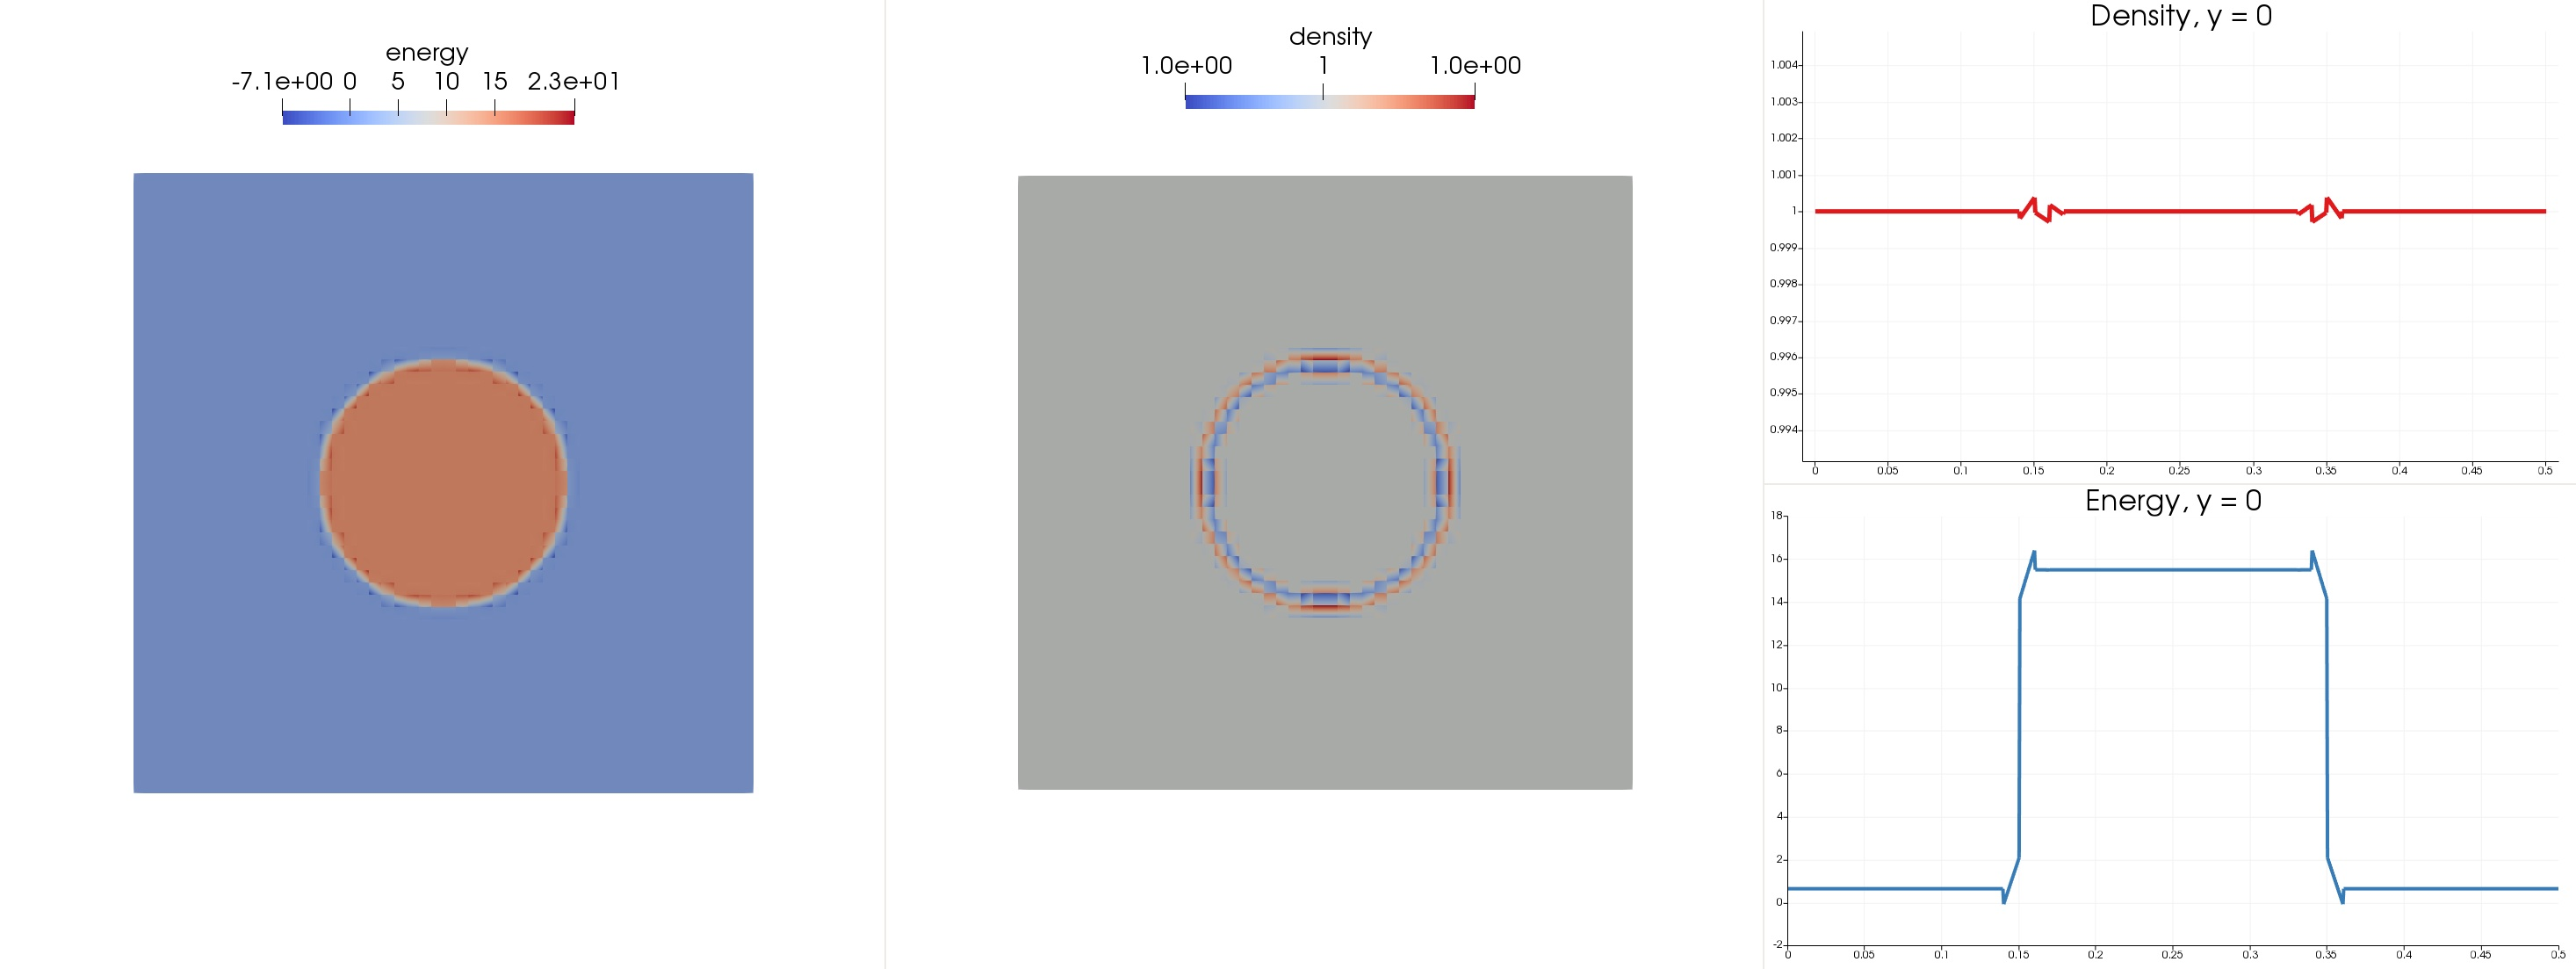
\includegraphics[width=0.82\textwidth]{img/limit/nl1.jpg}
		\end{center}
	\end{figure}\vspace{-12mm}
	\begin{figure}[H]
		\begin{center}
			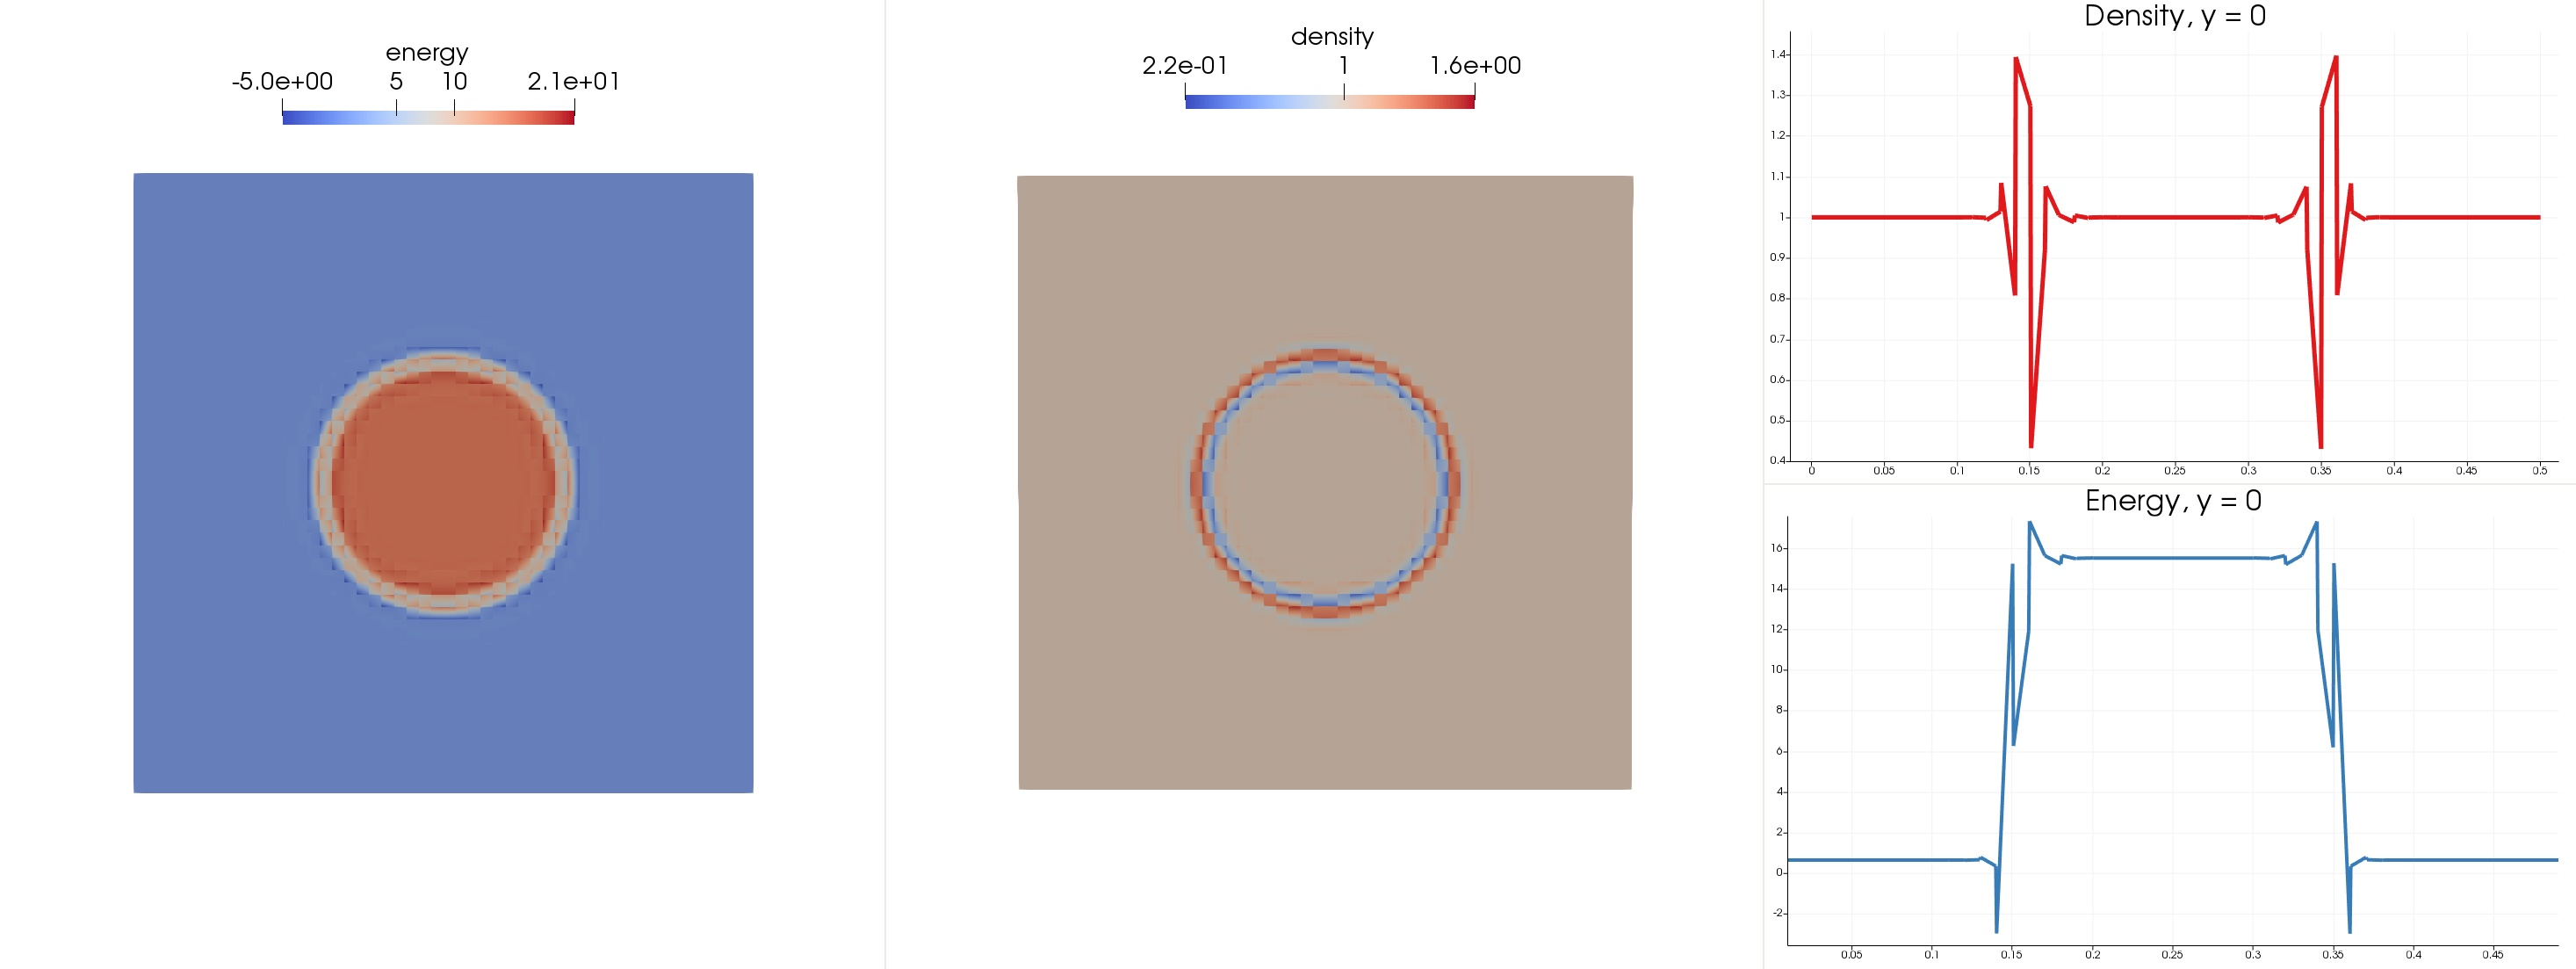
\includegraphics[width=0.82\textwidth]{img/limit/nl2.jpg}
		\end{center}
	\end{figure}\vspace{-12mm}
	\begin{figure}[H]
		\begin{center}
			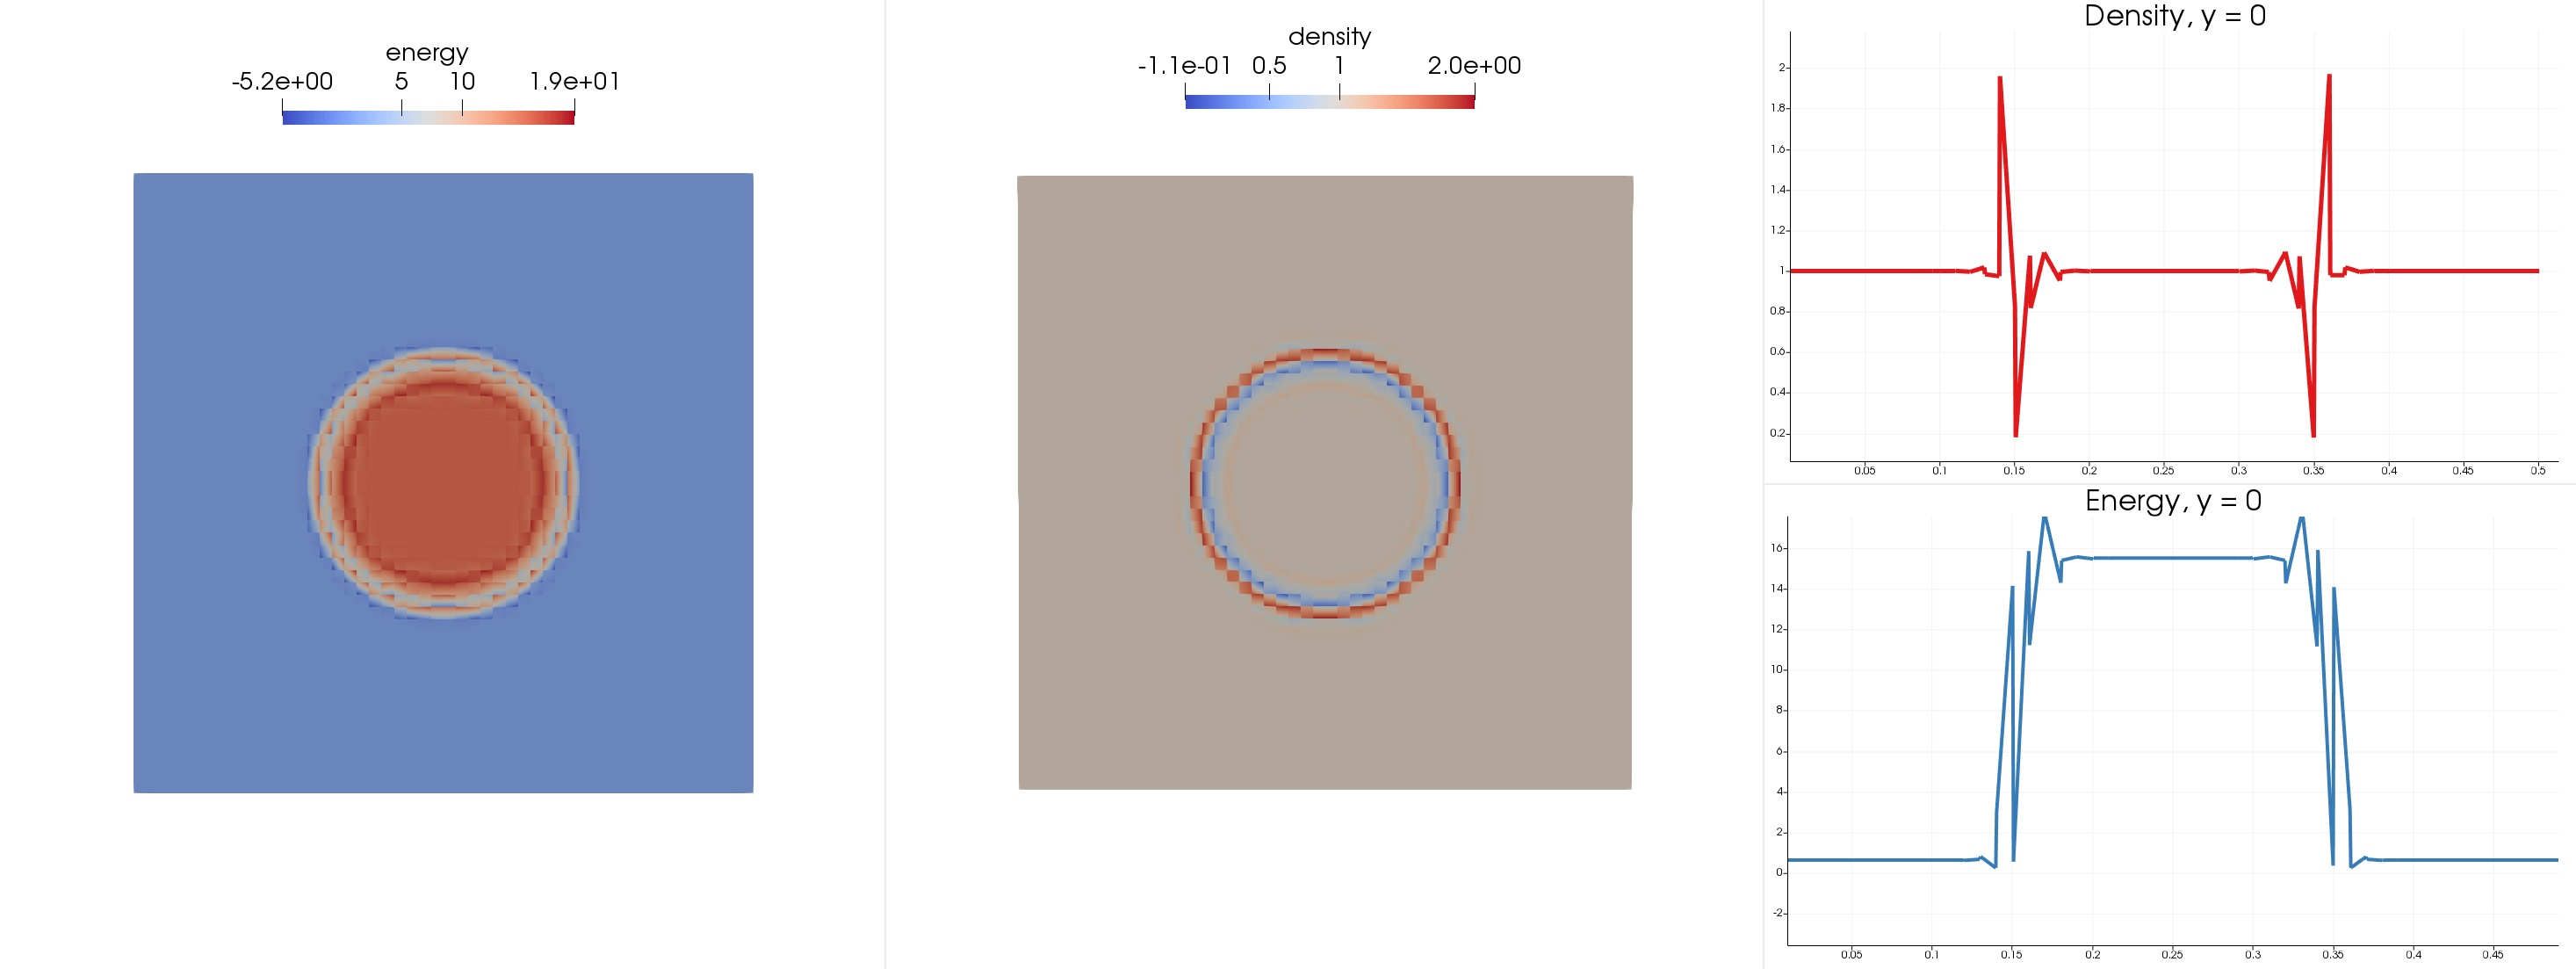
\includegraphics[width=0.82\textwidth]{img/limit/nl3.jpg}
		\end{center}
	\end{figure}\vspace{-12mm}
	\begin{figure}[H]
		\begin{center}
			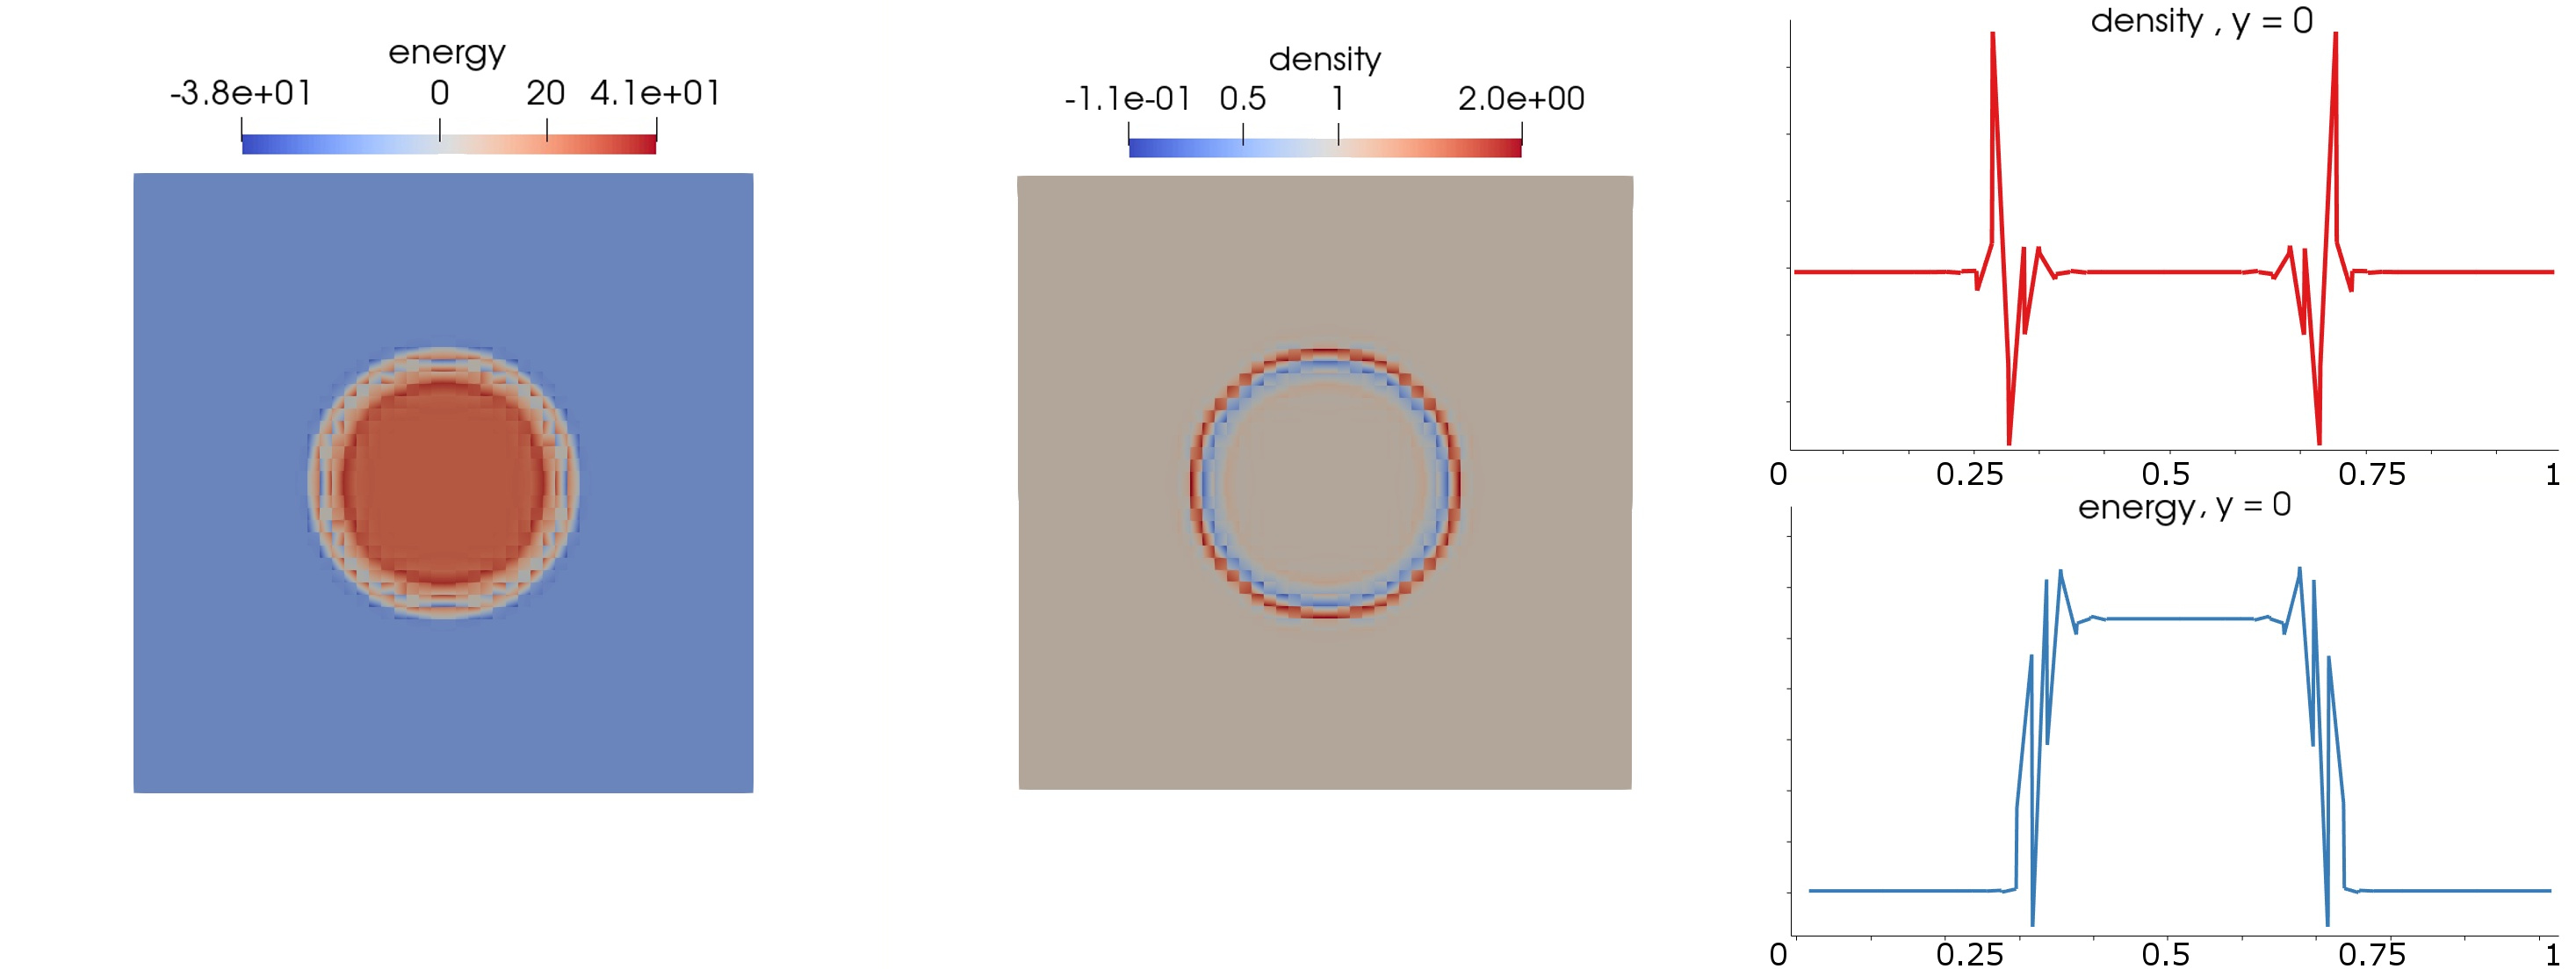
\includegraphics[width=0.82\textwidth]{img/limit/nl4.jpg}
		\end{center}
	\end{figure}\vspace{-12mm}
	\begin{figure}[H]
		\begin{center}
			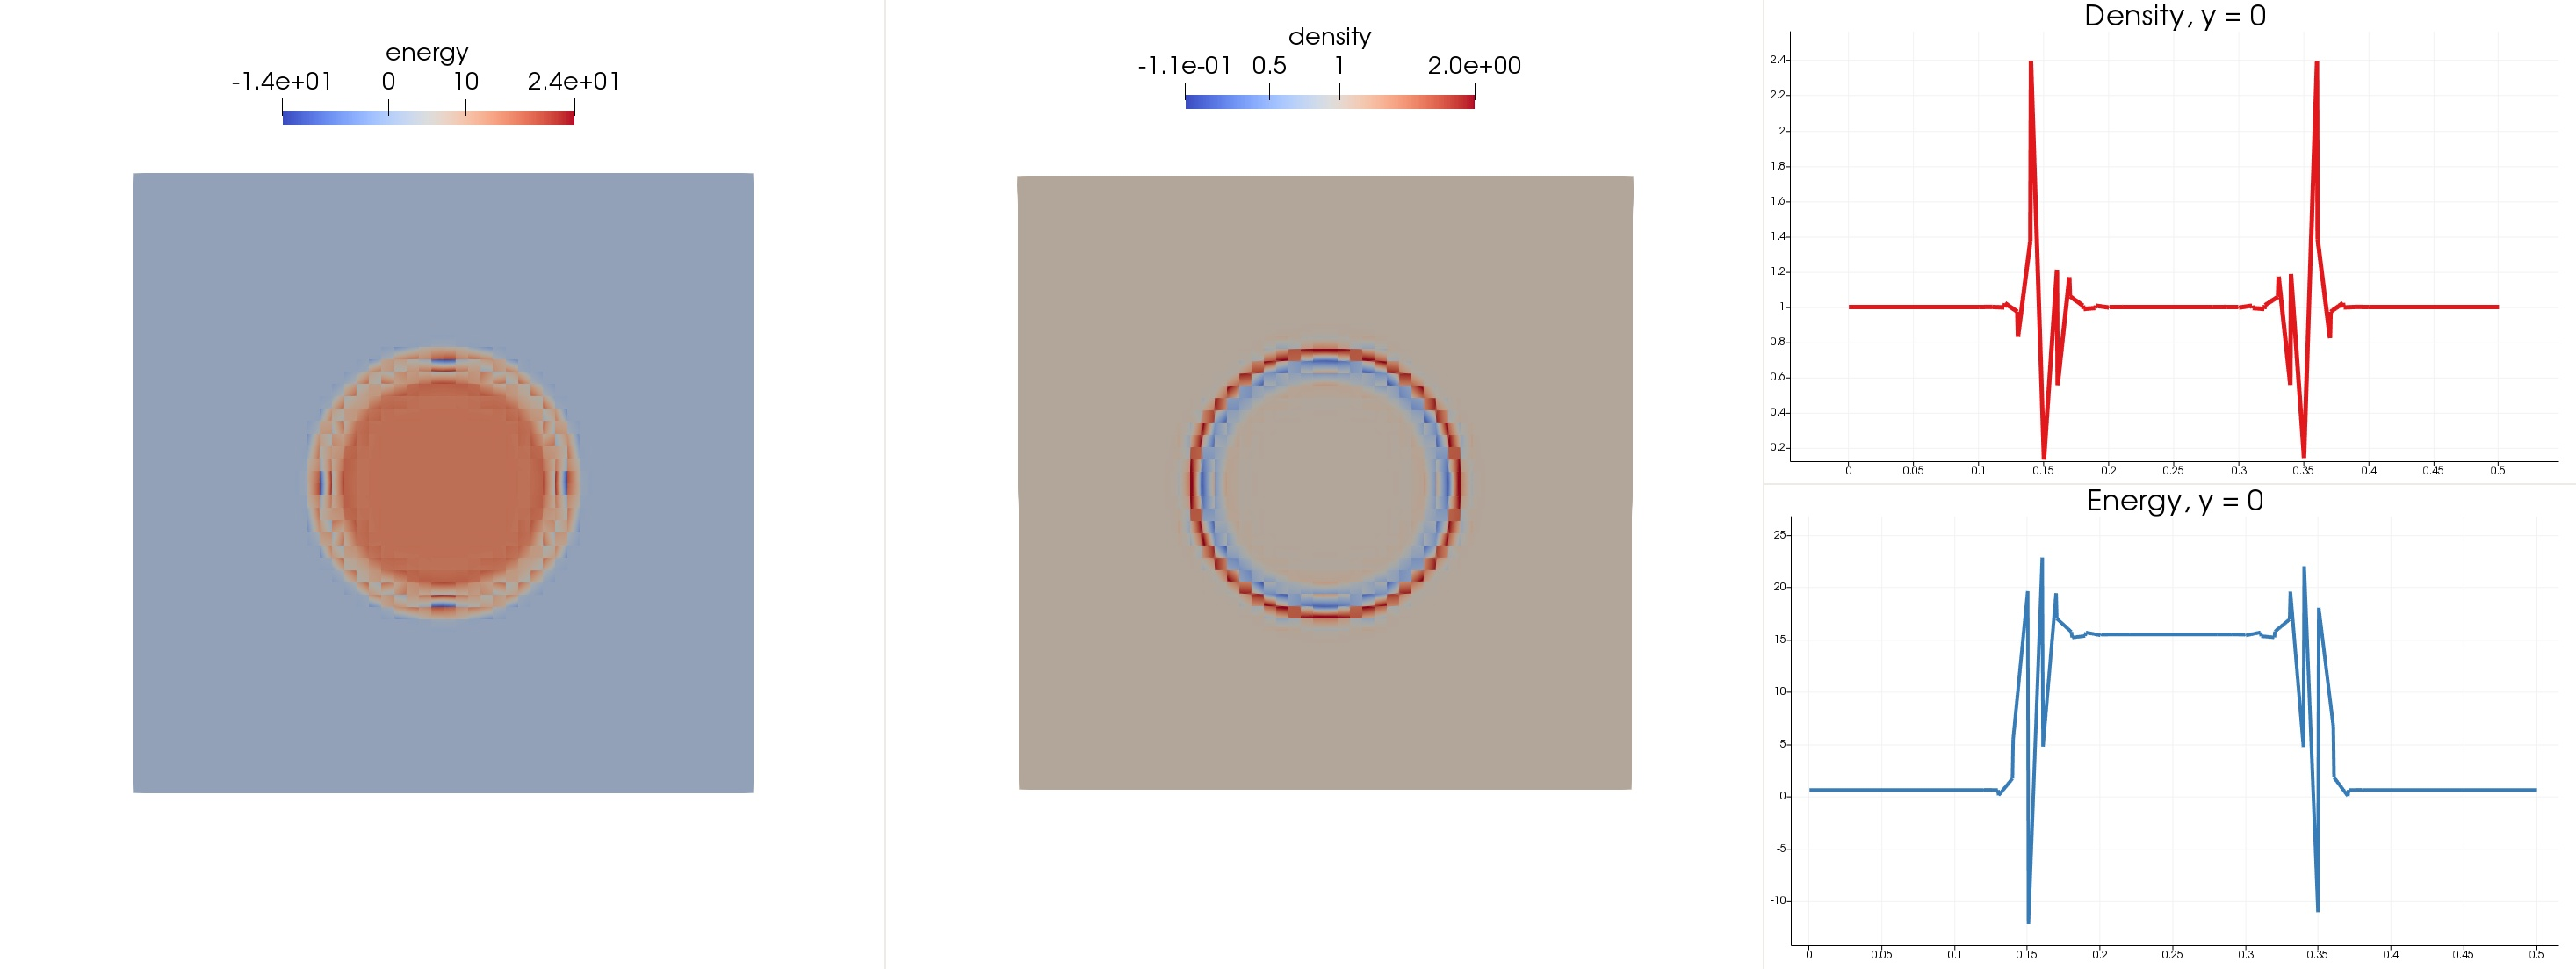
\includegraphics[width=0.82\textwidth]{img/limit/nl5.jpg}
		\end{center}
	\end{figure}\vspace{-12mm}
	\begin{figure}[H]
		\begin{center}
			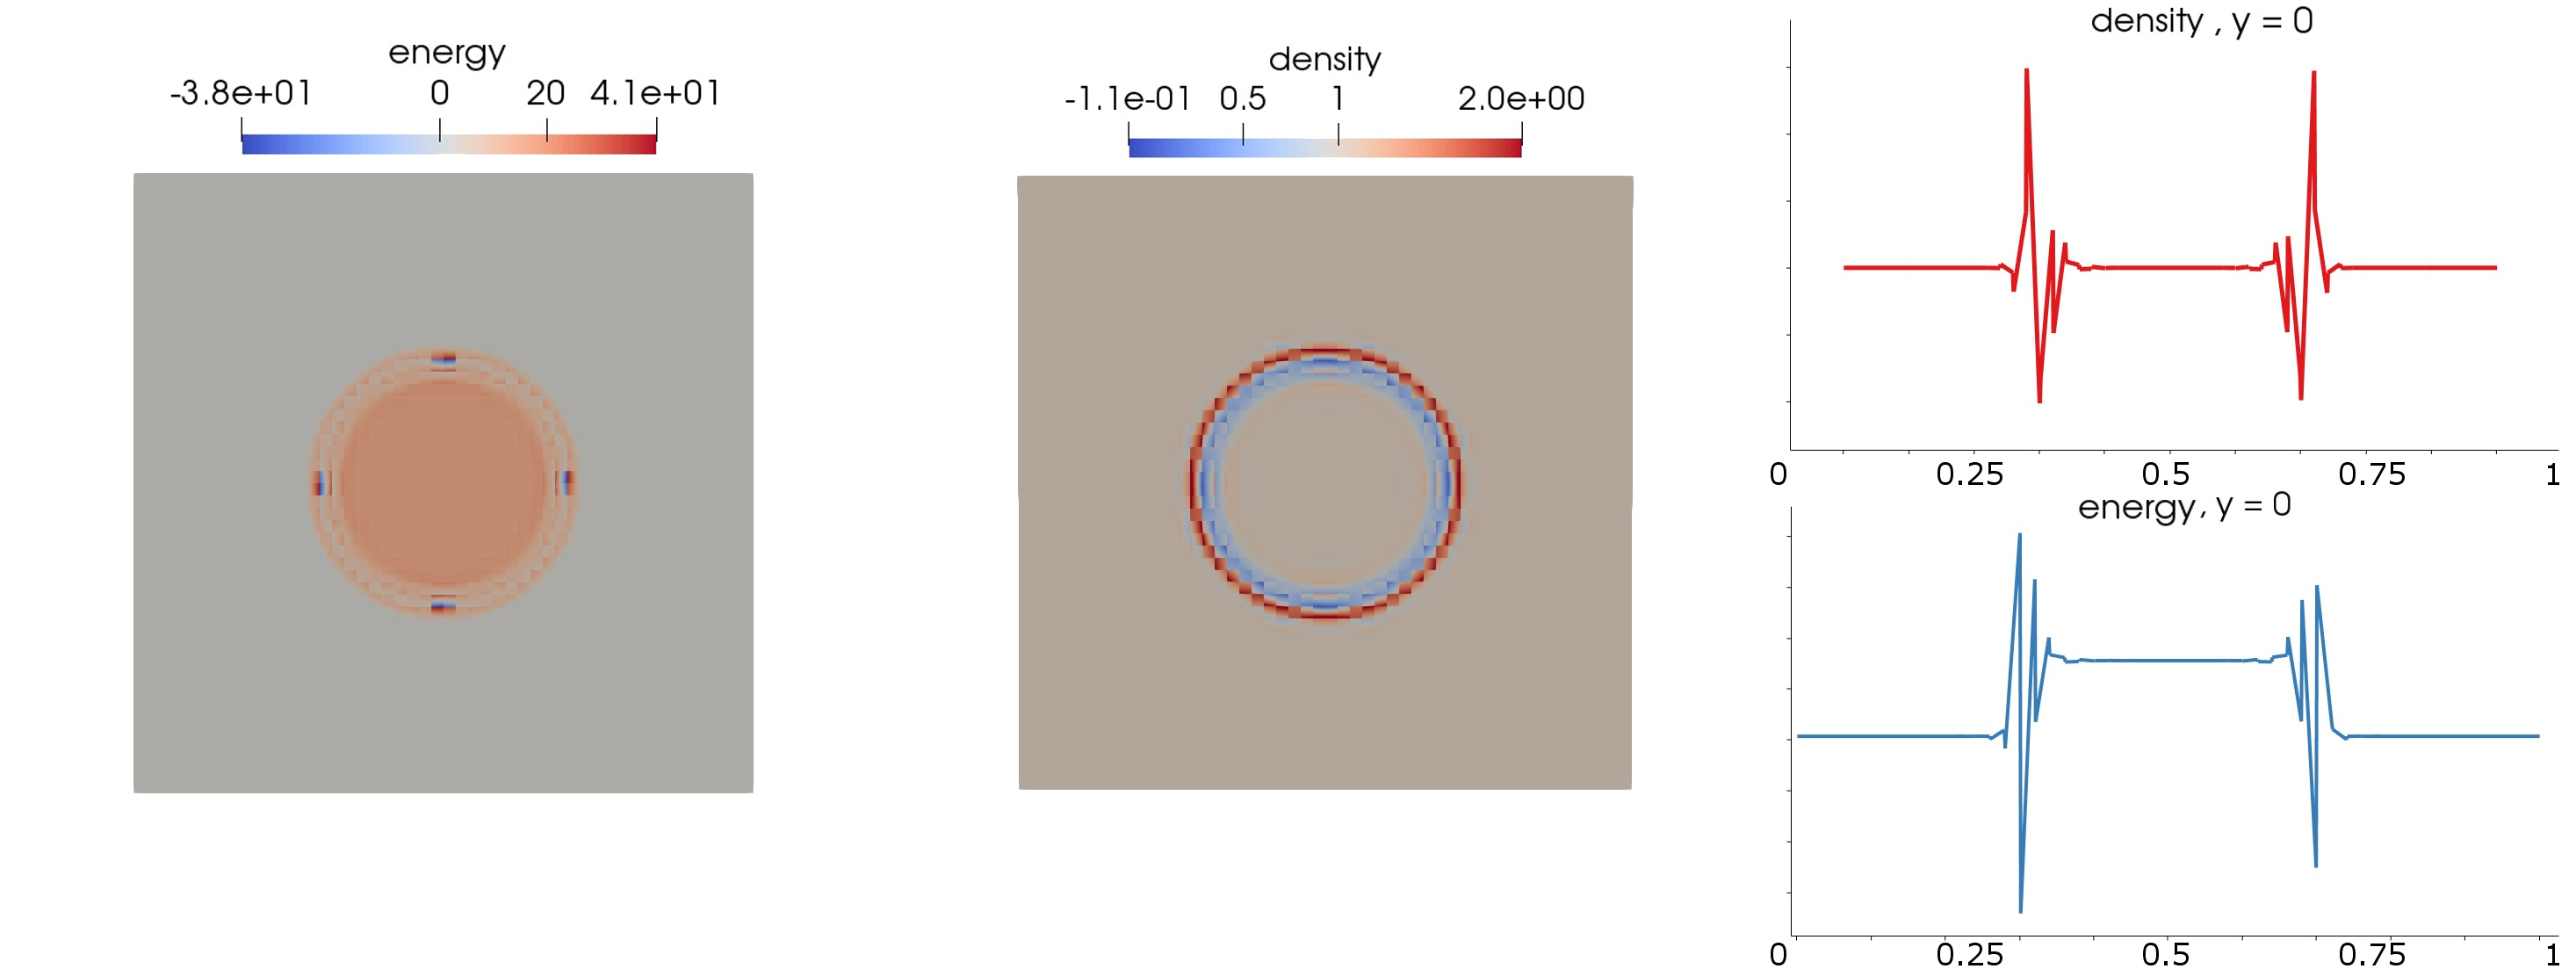
\includegraphics[width=0.82\textwidth]{img/limit/nl6.jpg}		
			\caption{Unlimited solution - Energy, density, and their values over line y = 0, the solution cannot progress beyond the last snapshot, as the oscillations are orders of magnitude larger than the physical solution}
		\end{center}
	\end{figure}
	
	\newpage
	
\begin{figure}[H]
		\begin{center}
			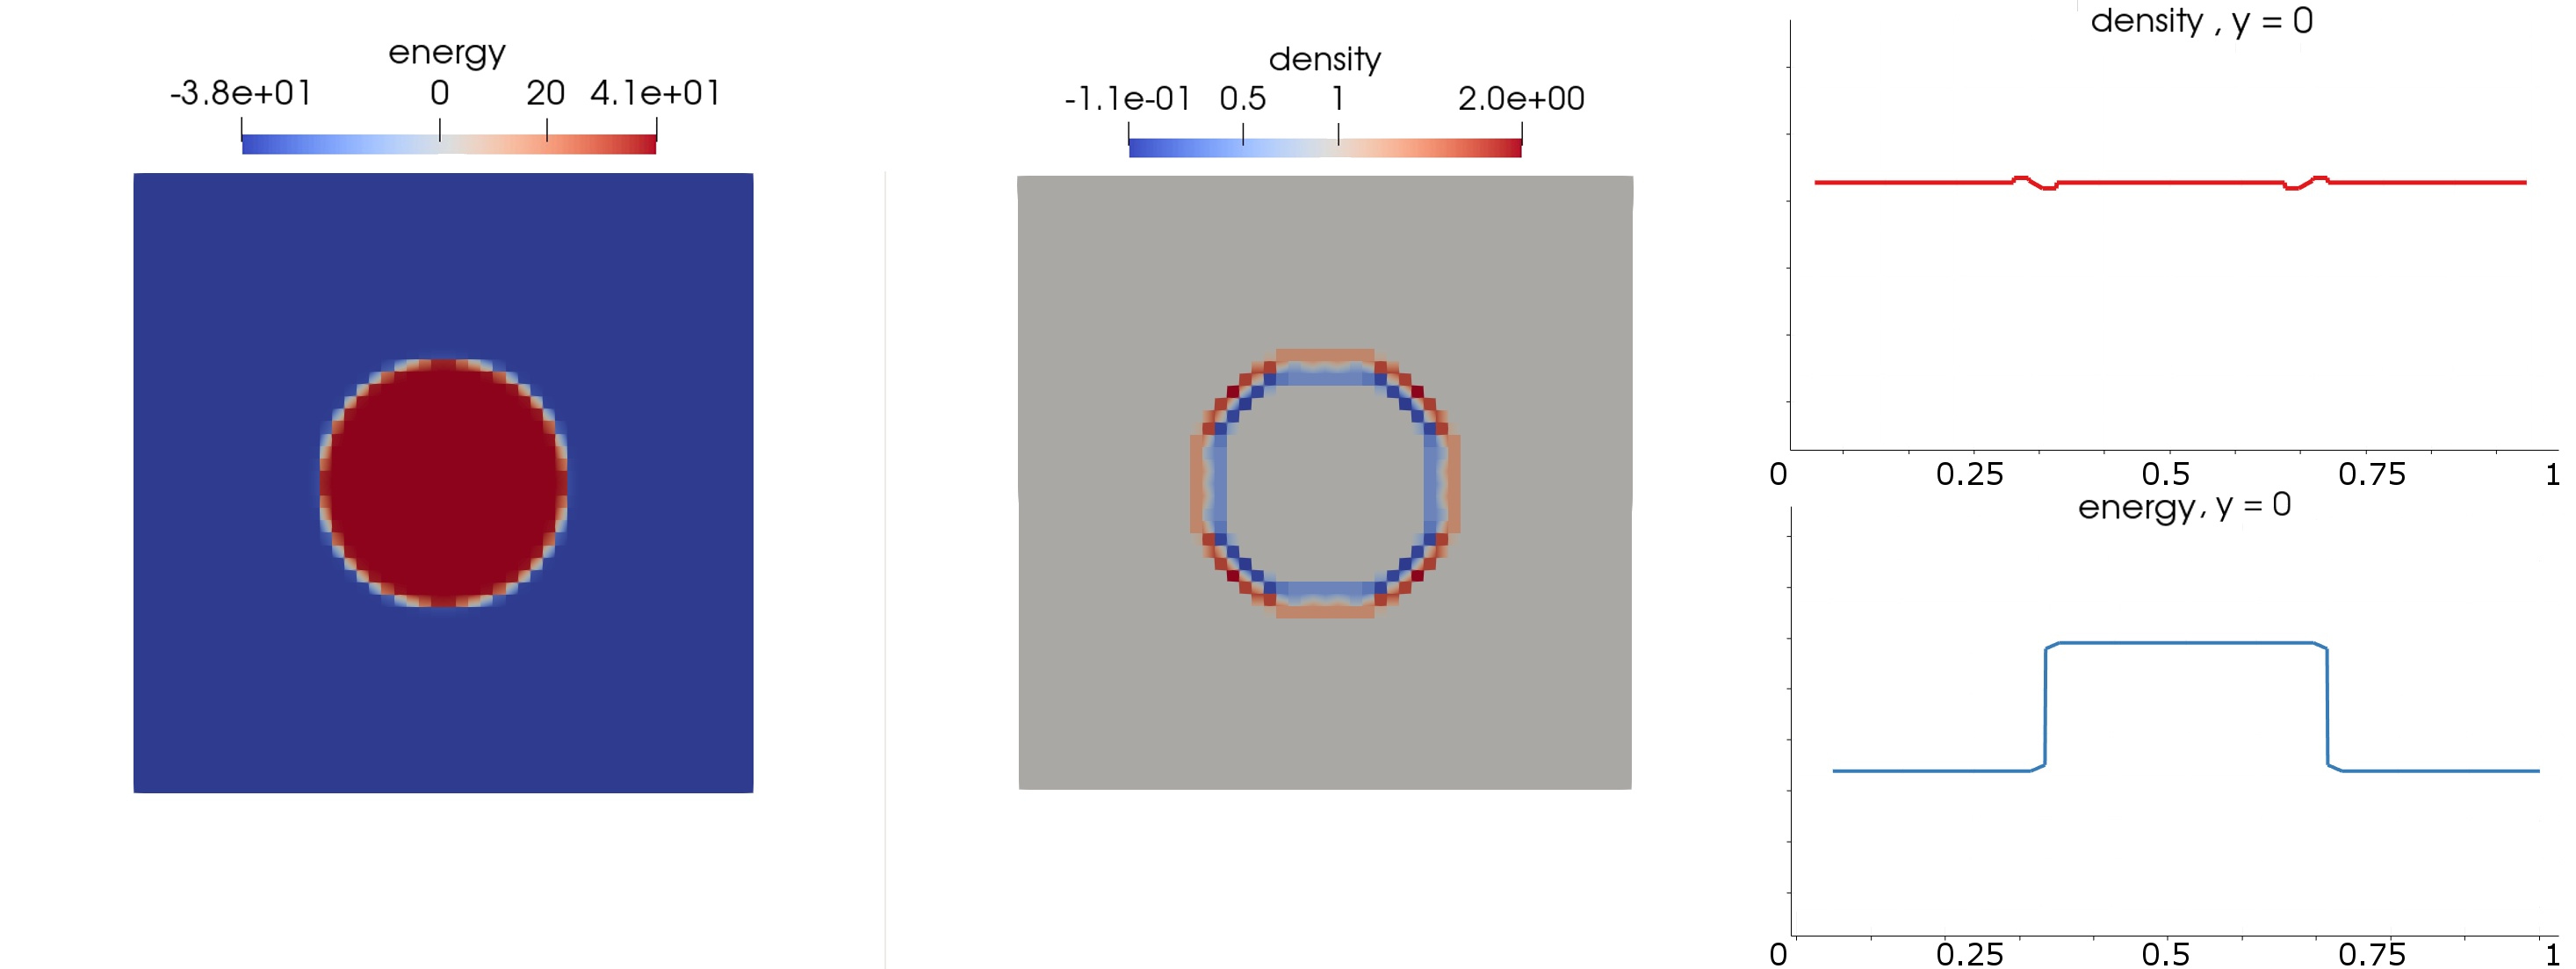
\includegraphics[width=0.82\textwidth]{img/limit/l1.jpg}
		\end{center}
	\end{figure}\vspace{-12mm}
	\begin{figure}[H]
		\begin{center}
			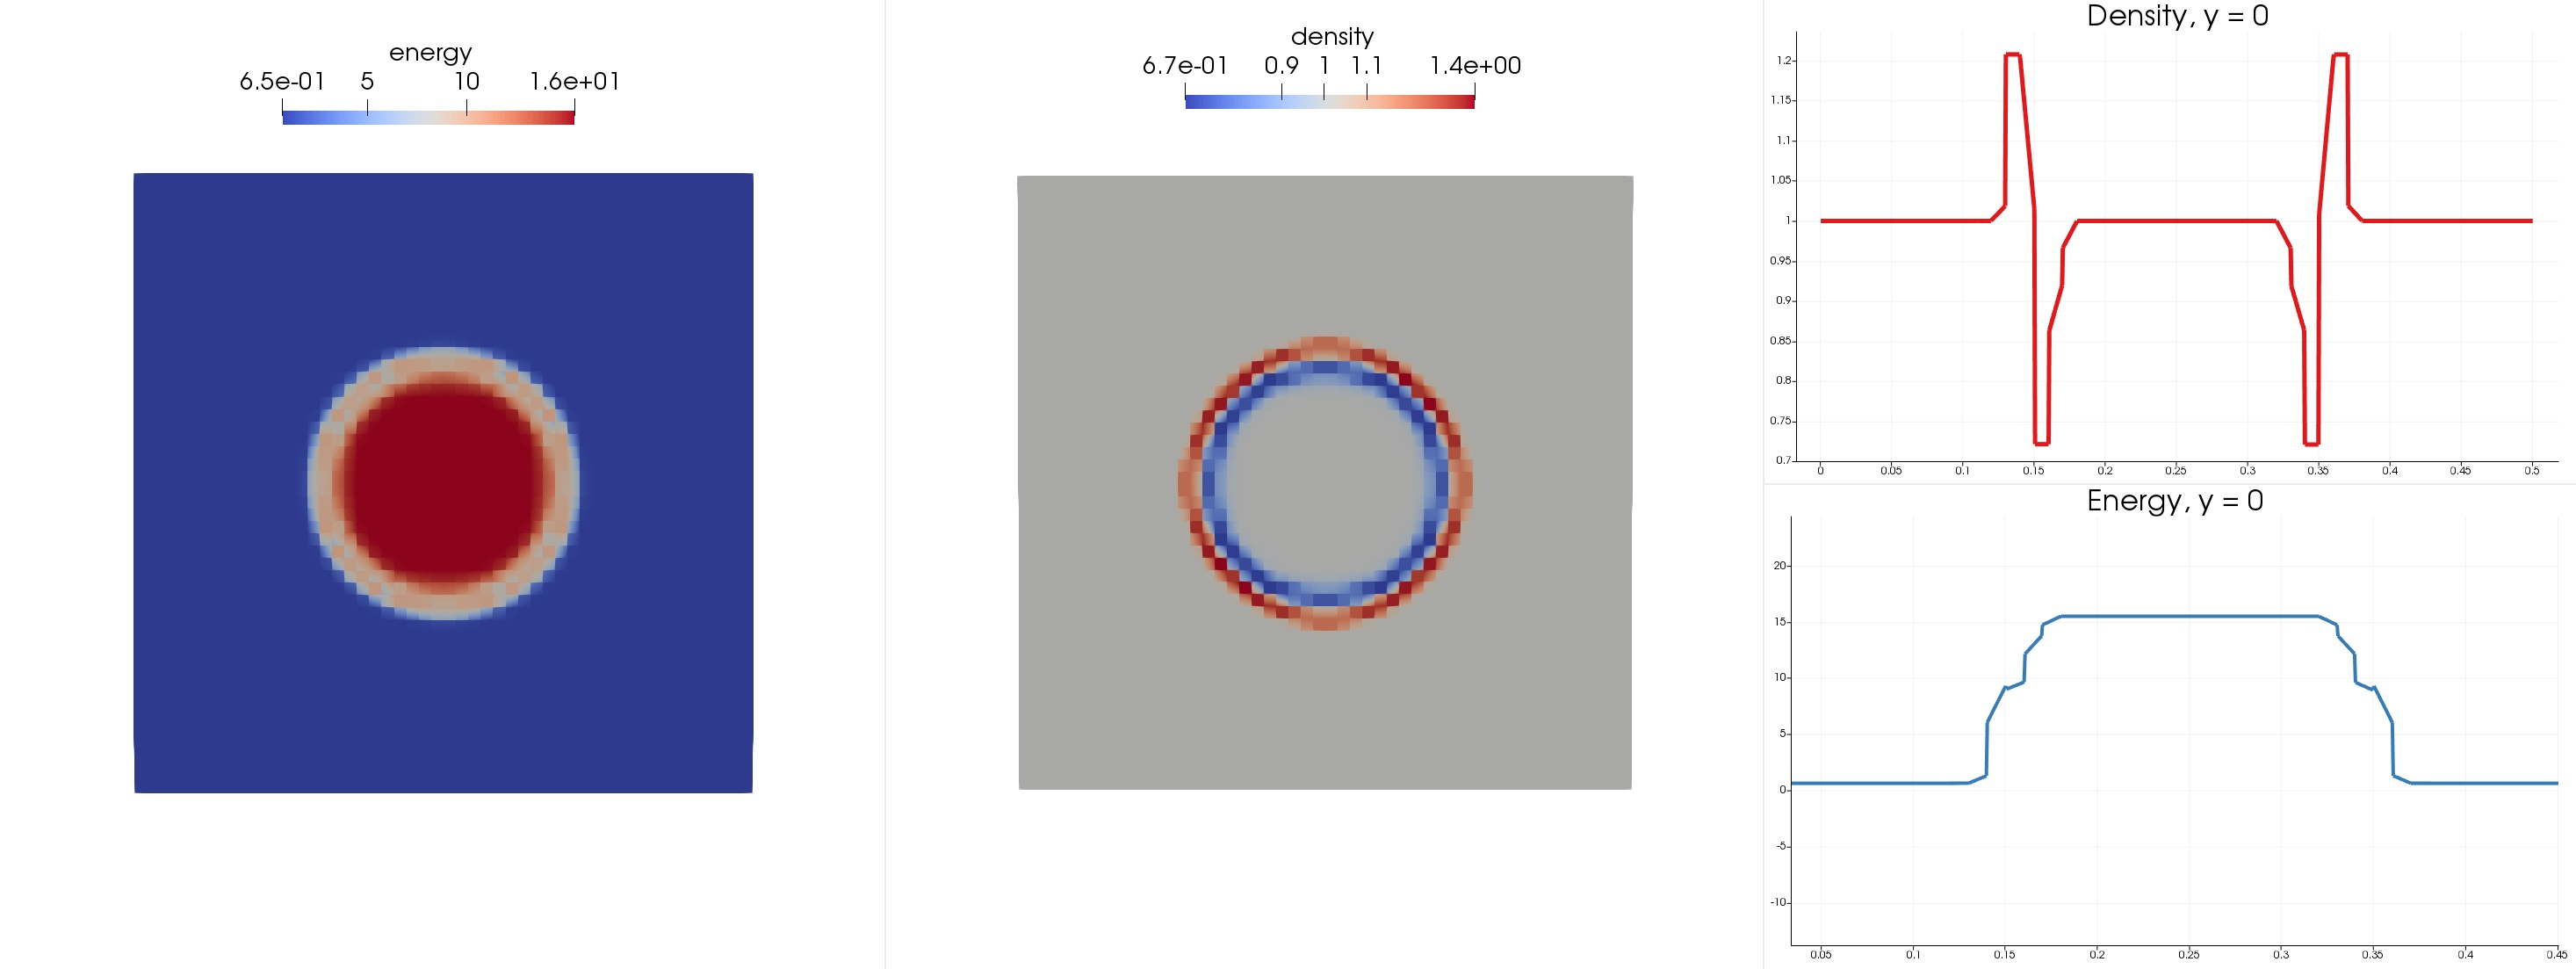
\includegraphics[width=0.82\textwidth]{img/limit/l2.jpg}
		\end{center}
	\end{figure}\vspace{-12mm}
	\begin{figure}[H]
		\begin{center}
			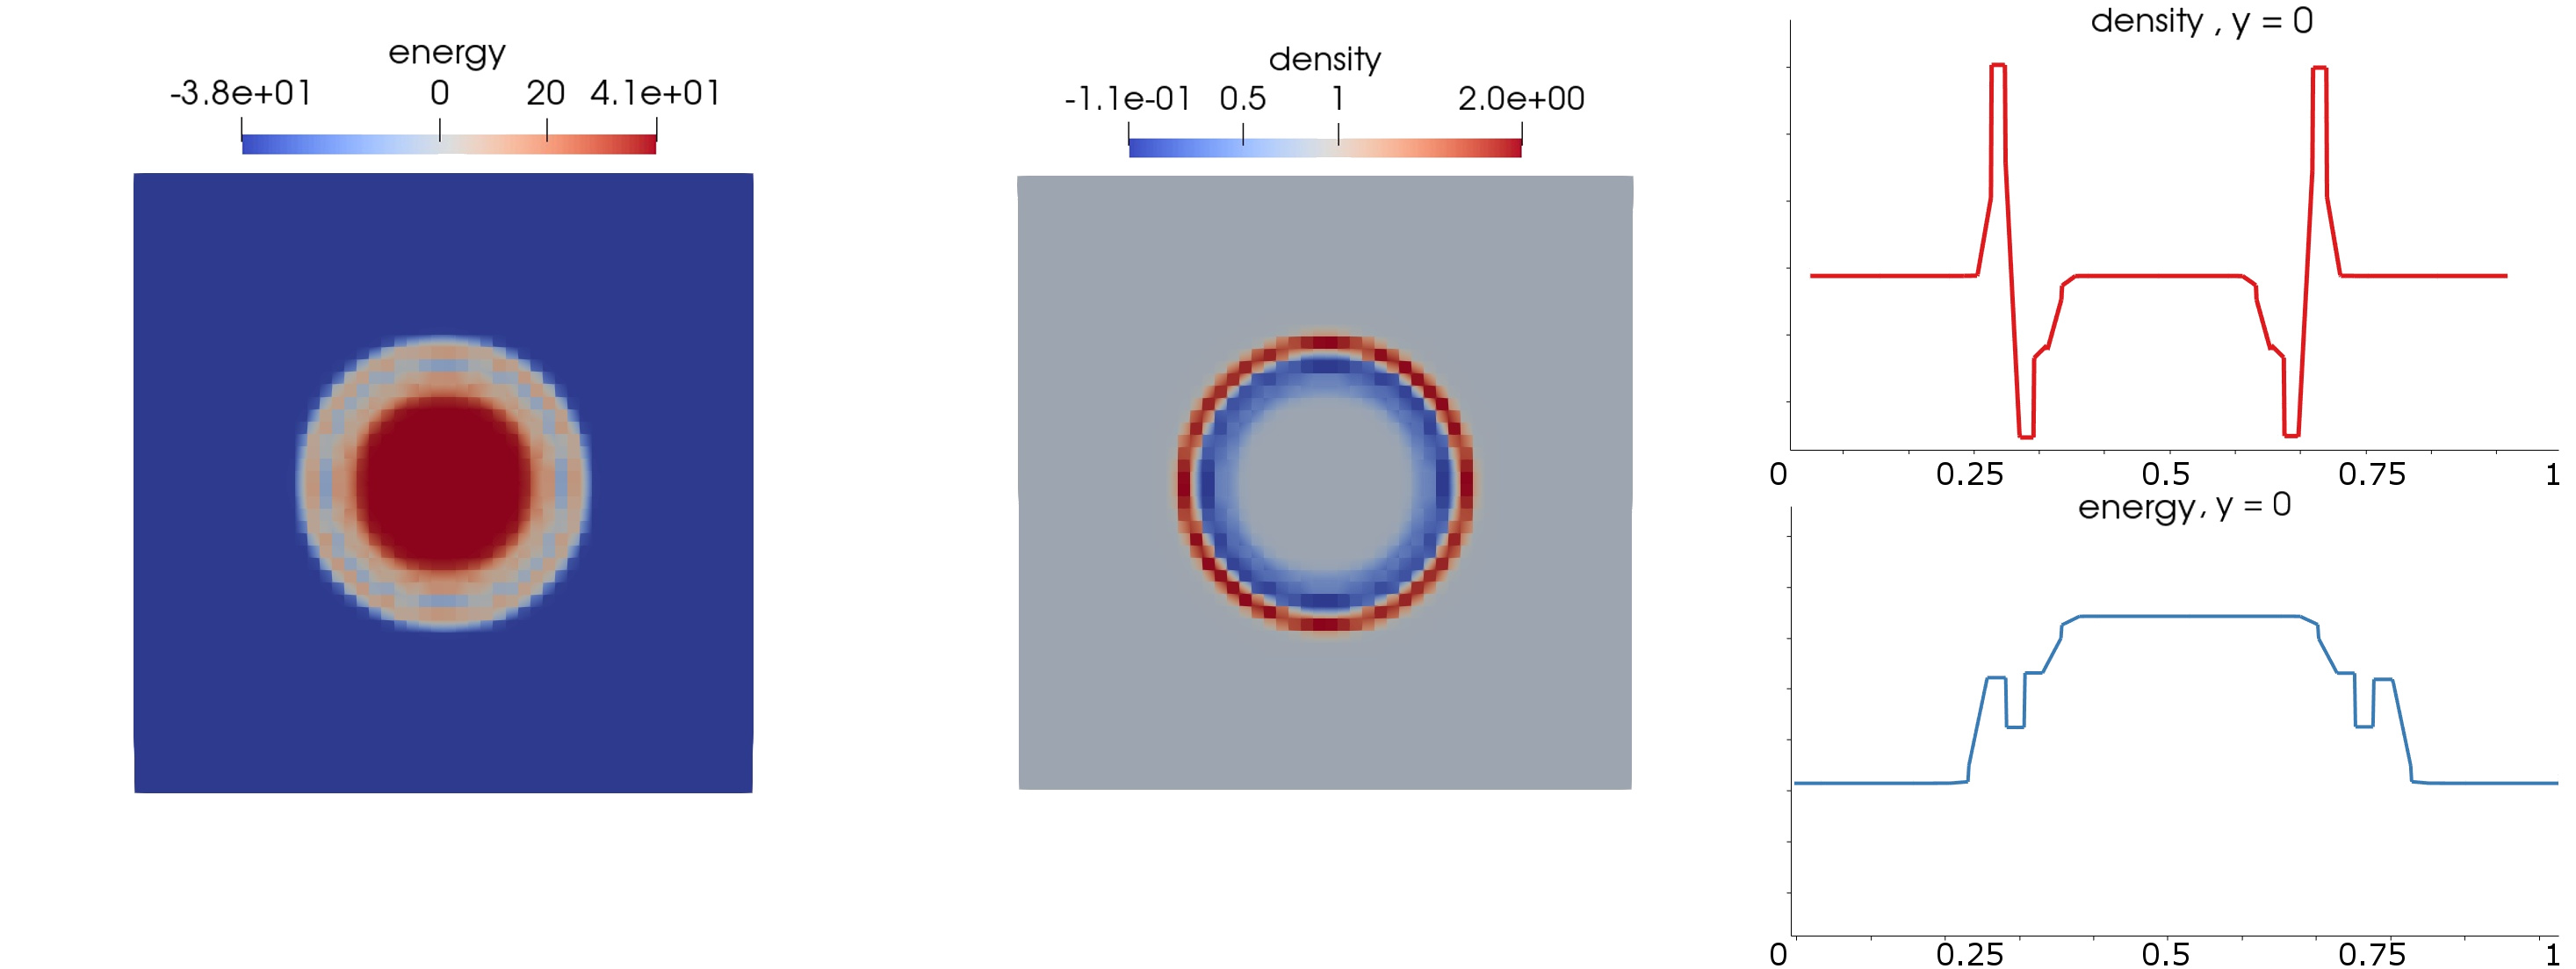
\includegraphics[width=0.82\textwidth]{img/limit/l3.jpg}
		\end{center}
	\end{figure}\vspace{-12mm}
	\begin{figure}[H]
		\begin{center}
			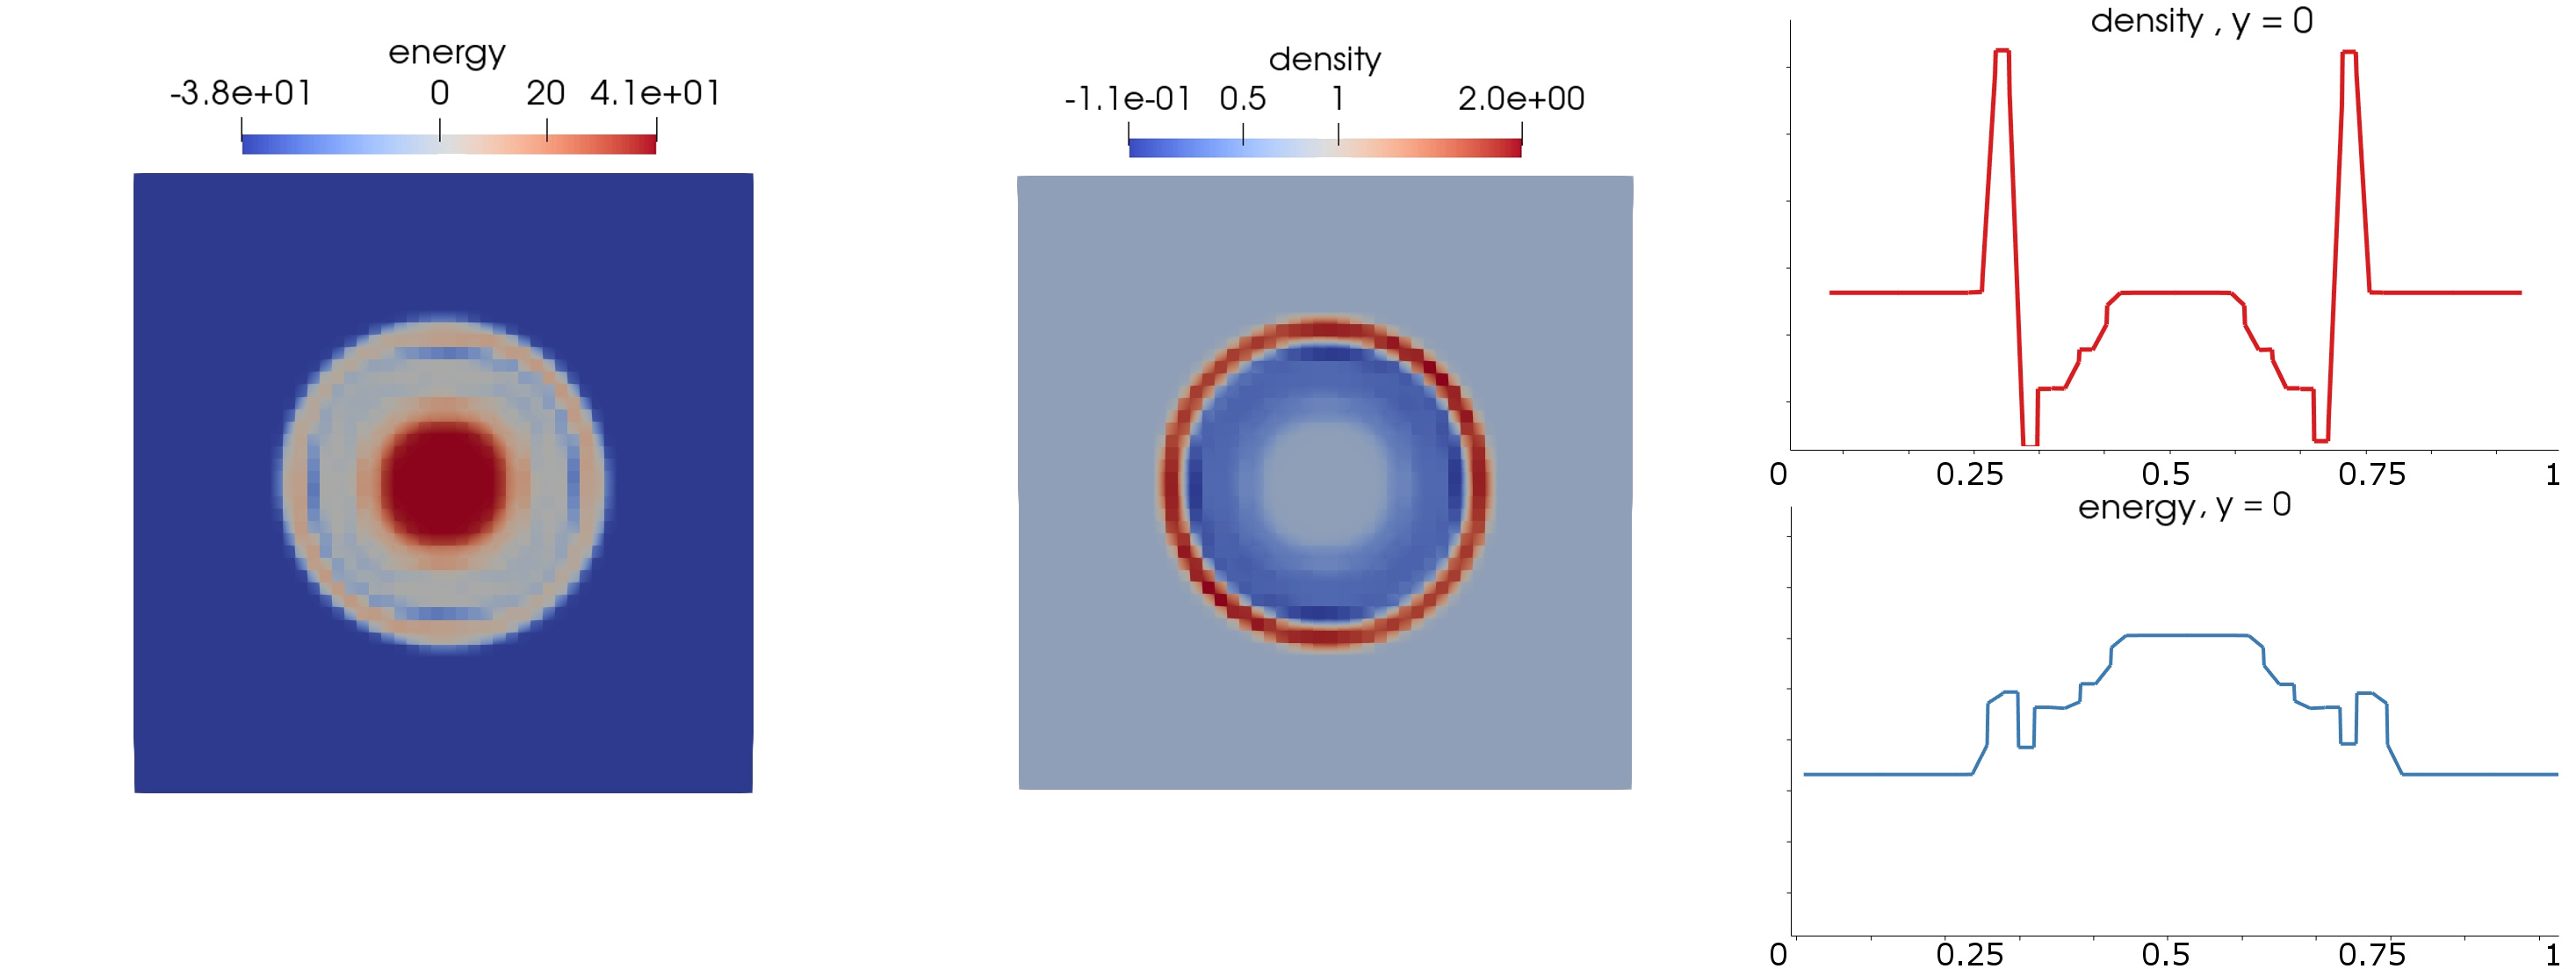
\includegraphics[width=0.82\textwidth]{img/limit/l4.jpg}
		\end{center}
	\end{figure}\vspace{-12mm}
	\begin{figure}[H]
		\begin{center}
			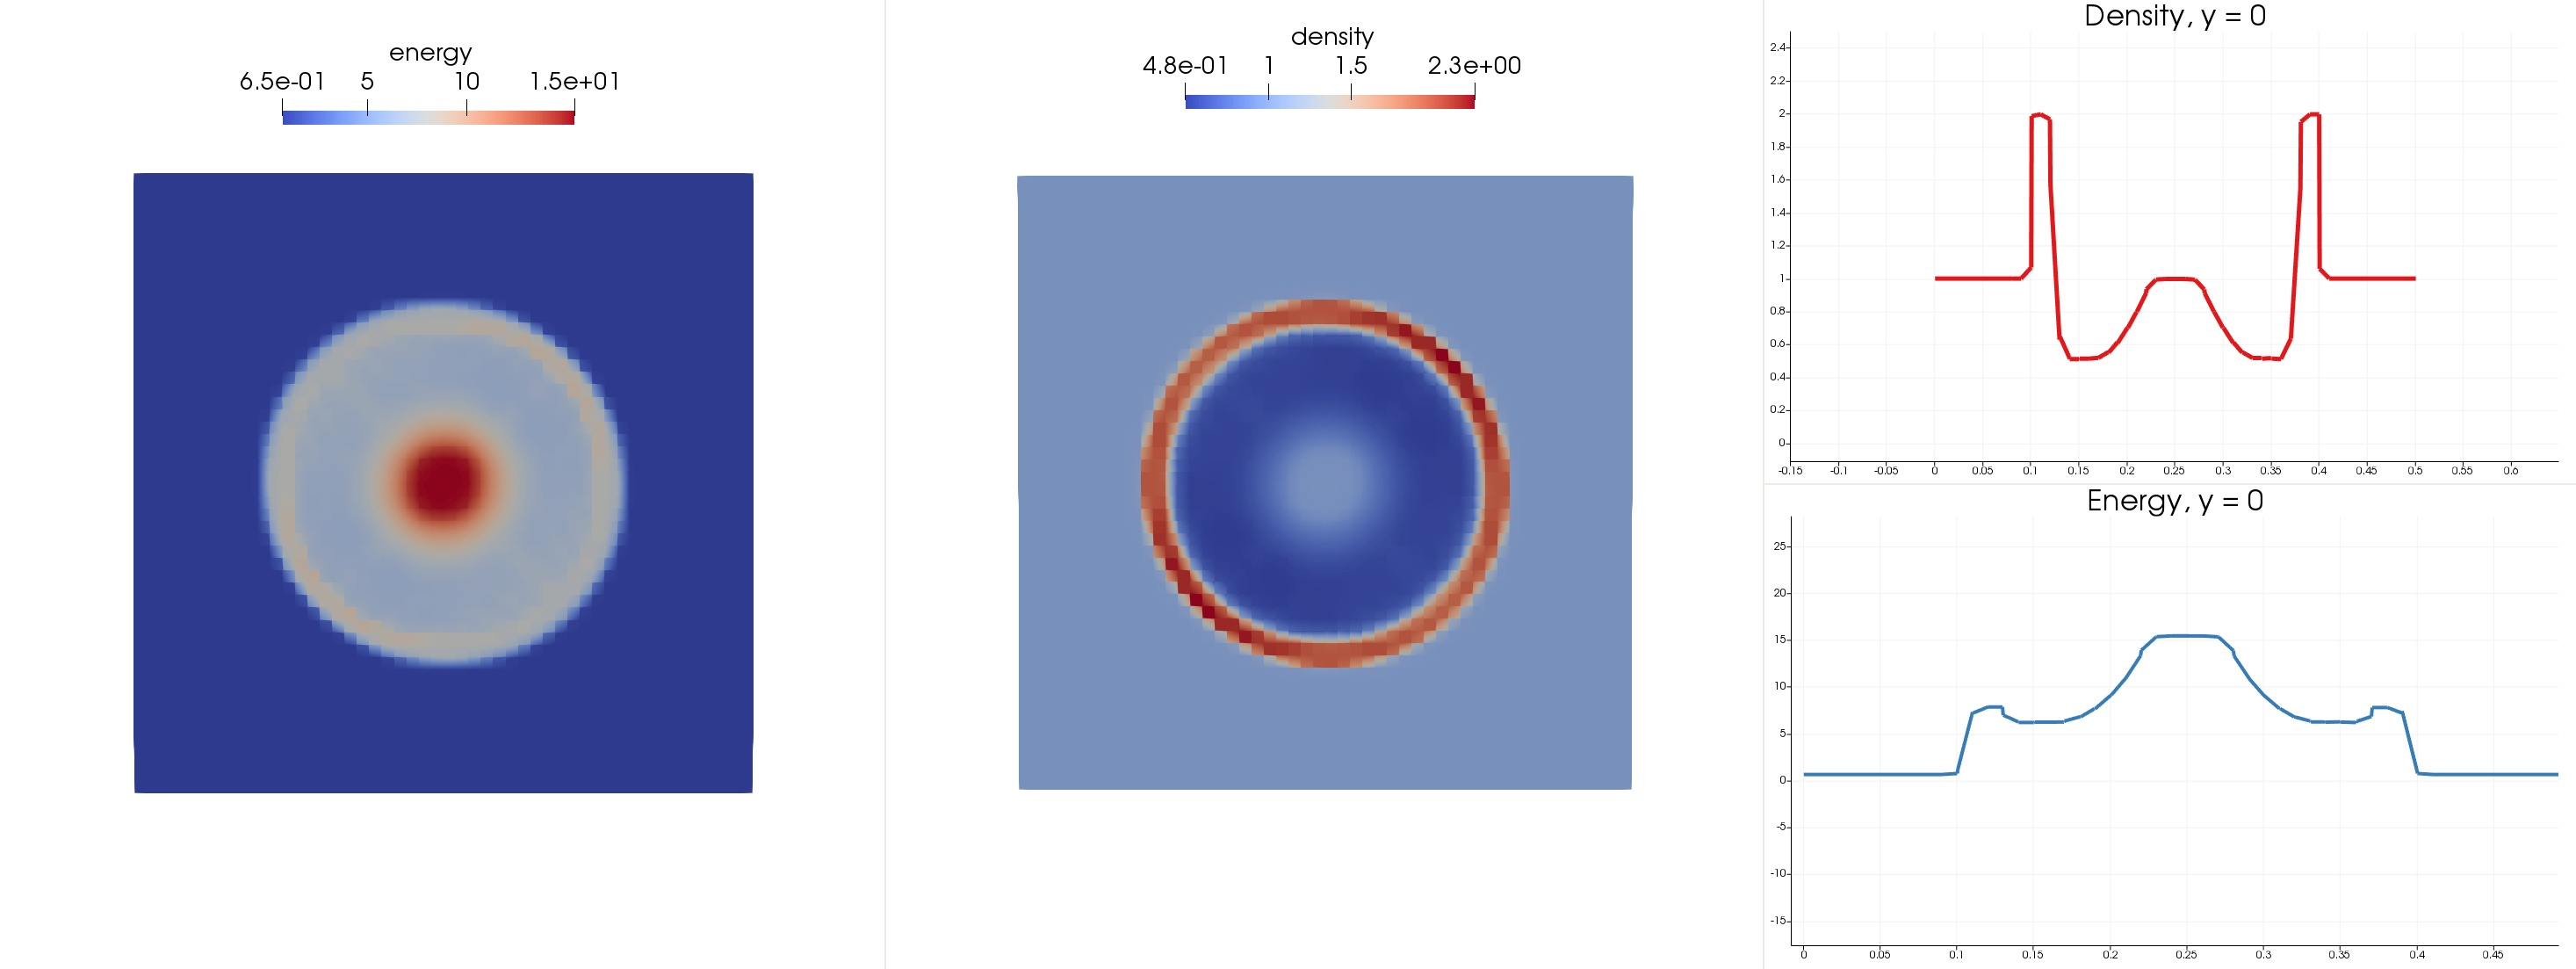
\includegraphics[width=0.82\textwidth]{img/limit/l5.jpg}
		\end{center}
	\end{figure}\vspace{-12mm}
	\begin{figure}[H]
		\begin{center}
			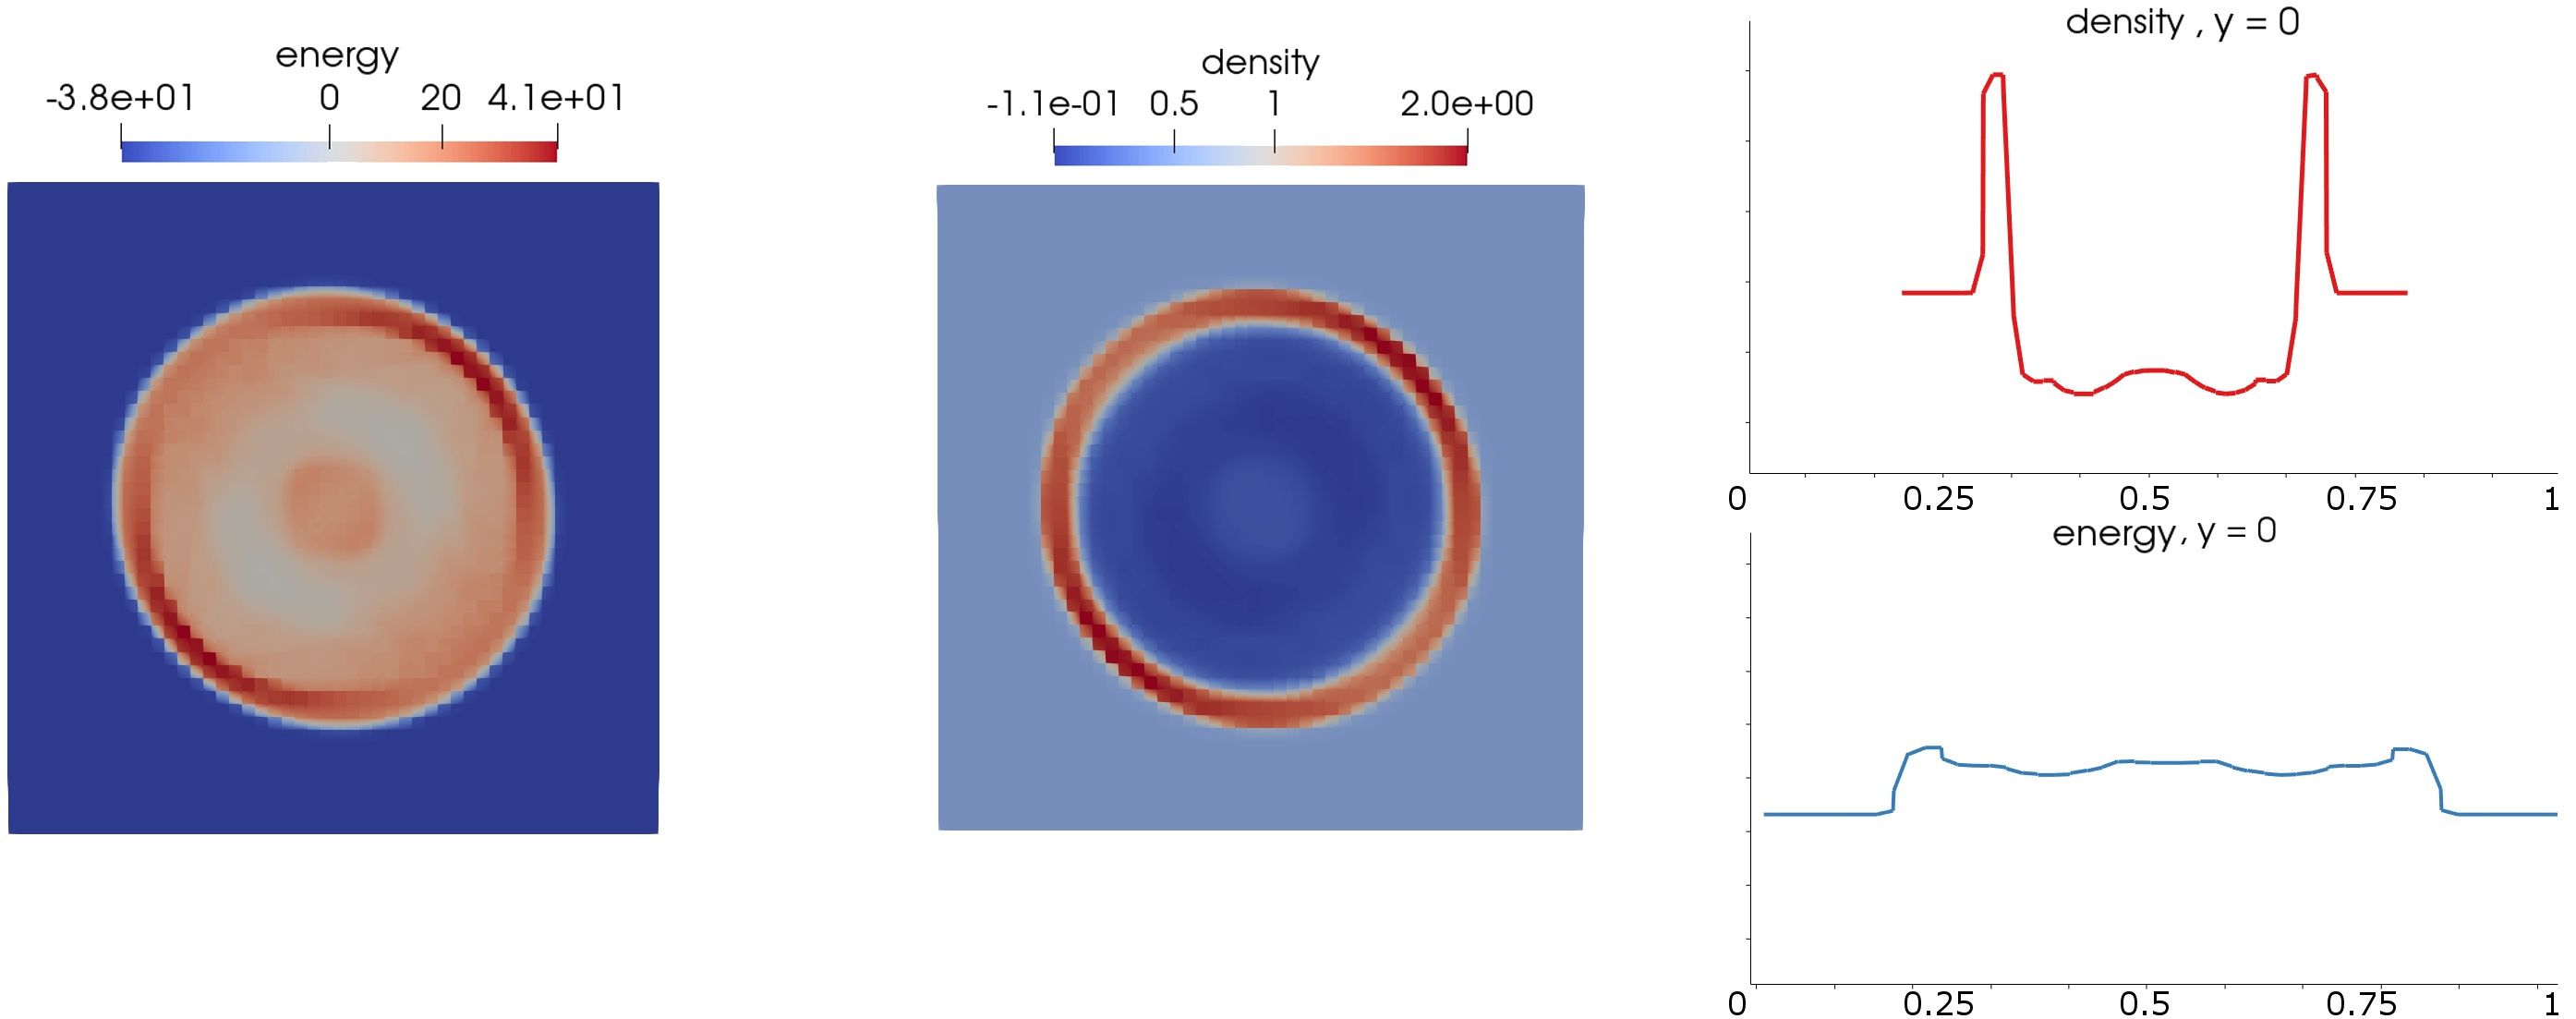
\includegraphics[width=0.82\textwidth]{img/limit/l6.jpg}
			\caption{Solution limited with Vertex-based limiter - Energy, density, and their values over line y = 0}
		\end{center}
	\end{figure}
